% !TeX encoding = UTF-8
% !TeX spellcheck = en_US
% !BIB TS-program = biber
% basic packages and document settings
\documentclass[a4paper,14pt]{article}
\usepackage[english]{babel}
\usepackage[utf8]{inputenc}
\usepackage[T1]{fontenc}
\usepackage[a4paper]{geometry}
\geometry{top = 30mm, bottom = 25mm, left = 25mm, right = 25mm,  bindingoffset=1cm}
\usepackage{setspace}
\onehalfspacing
\raggedbottom
\pdfcompresslevel9

% mathmode-related packages
\usepackage{mathtools}
\usepackage{physics}
\usepackage{amsmath}
\usepackage{amsthm}
\usepackage{amsbsy}
\usepackage{mathrsfs}
\usepackage{amssymb}
\usepackage{amstext}
\usepackage{amsfonts}
\usepackage{tikz}
\usepackage{siunitx}
%\usepackage{IEEEtrantools}

% misc
\usepackage{esdiff}
\usepackage{multirow}
\usepackage{blindtext}
\usepackage{todonotes}
\usepackage{abstract}
\usepackage{appendix}
\usepackage[bottom]{footmisc}
\usepackage{listings}

% packages requiring setup arguments


% graphics and floats
\usepackage{graphicx}
\graphicspath{{../Figures/},{../Figures/intro/},{../Figures/res-tracking/},{../Figures/dephasing/},{../Figures/relaxation/}}
\usepackage{float}
\usepackage{wrapfig}
%\usepackage{subfloat}
\usepackage{subcaption}
%\usepackage{caption}
\usepackage[rightcaption]{sidecap}
\usepackage{tabularx}
\usepackage{adjustbox}
\usepackage{svg}
\usepackage{epstopdf}
\usepackage{grffile}	% handle file names with dots, spaces etc.
%\usepackage{flafter}
\usepackage{rotating}
%\usepackage{floatrow}
%\floatsetup[figure]{capposition=beside,capbesideposition={top,right}}

%\usepackage{epstopdf}
%\epstopdfDeclareGraphicsRule{.pdf}{png}{.png}{convert #1 \OutputFile}
%\AppendGraphicsExtensions{.pdf}

\usepackage{xcolor}
%\definecolor{rwth-dark}{HTML}{176daf}
\definecolor{rwth-dark}{RGB}{0,84,159}
%\definecolor{rwth-light}{HTML}{8abae3}
\definecolor{rwth-light}{RGB}{142,186,229}

%/**
%* Generated by Gpick 0.2.5
%* RWTH Dark: #176daf, rgb(23, 109, 175), hsl(32, 43%, 69%)
%* RWTH Light: #8abae3, rgb(138, 186, 227), hsl(195, 73%, 89%)
%*/

\usepackage{hyperref}
\hypersetup{hidelinks=true,colorlinks=true,allcolors=rwth-dark}
\usepackage[nameinlink,capitalise]{cleveref}
%\usepackage[hyphens]{url}
%\urlstyle{sf}
%\usepackage{breakurl}


% header & footer settings
\usepackage{fancyhdr}
\pagestyle{fancy}
%\renewcommand{\chaptermark}[1]{\markboth{#1}{}} % with this we ensure that the chapter and section headings are in lowercase.
\renewcommand{\sectionmark}[1]{\markright{\thesection\ #1}}
\fancyhf{} % delete current header and footer

\fancyhead[LE,RO]{\large\thepage}
\fancyhead[LO]{\large\rightmark}
\fancyhead[RE]{\large\leftmark}

\renewcommand{\headrulewidth}{0.3pt}
\renewcommand{\footrulewidth}{0pt}
%\addtolength{\headheight}{0.5pt} % space for the rule

\fancyfoot[C]{\thepage}

\fancypagestyle{plain}
{
	\fancyhead{} % get rid of headers on plain pages
	\renewcommand{\headrulewidth}{0pt} % and the line
}

% ========== command definitions =================================
\newcommand{\Thickline}{\rule{\linewidth}{0.4mm}}
\newcommand{\Thinline}{\rule{\linewidth}{0.1mm}}

\newcommand{\id}{\, \mathrm{d}}

\definecolor{codegray}{gray}{0.9}
\newcommand{\code}[1]{\colorbox{codegray}{\texttt{#1}}}

\newcommand{\skippage}{\clearpage{\thispagestyle{empty}\cleardoublepage}}

\def\@esphack{%
	\relax
	\ifhmode
	\spacefactor\@savsf
	\ifdim\@savsk>\z@
	\ignorespaces
	\fi
	\fi}

\title{\LARGE title}
\date{}


\begin{document}
	
\begin{titlepage}
	\thispagestyle{empty}
	\newgeometry{top=20mm, left=20mm, right=20mm, bottom=20mm}
	
%	\begin{minipage}{0.35\textwidth}
%		\begin{flushleft}
%
%
%		\end{flushleft}
%	\end{minipage}
%	\hfill
%	\begin{minipage}{0.65\textwidth}
%		\begin{flushright}
%
%		\end{flushright}
%	\end{minipage}
	
	\vspace{3cm}
	\begin{center}
		\Thickline
		\vskip -0.45cm
		\Thinline
		\vspace{0.5cm}
		
		\huge{ \textbf{ title } } 
		
		\Thinline
		\vskip -1cm
		\Thickline 
		\vspace{1cm}

		
	\end{center}
	\vfill
	
\end{titlepage}
	
	
	
\skippage
\pagenumbering{roman}
\thispagestyle{plain}

\tableofcontents
%	\newpage
\listoffigures

\begingroup
\let\cleardoublepage\relax
\let\clearpage\relax
\listoftables
\endgroup
%\listoftables

\skippage

\pagenumbering{arabic}
\setcounter{page}{1}
\restoregeometry
\thispagestyle{fancy}

\skippage
	
\section{Einleitung}
Ziel dieses Versuchs ist die Aufnahme der Röntgenspektren verschiedener Materialien und die Bestimmung der enthaltenen Materialien. Dazu werden wir zwei unterschiedliche Aufbauten verwenden. Als erstes nutzen wir eine Americiumquelle (Am) um das untersuchte Material mit Alphastrahlung zu bescheßen und Röntgenstrahlen zu erzeugen. Später nutzen wir eine Röntgenröhre um das Material anzustrahlen.

\section{Theorie}
\subsection{Röntgenstrahlung}
Es gibt zwei Arten von Röntgenstrahlung: Bremsstrahlung, ein kontinuieriches Spektrum und charakteristische Strahlung, ein diskretes Spektrum.
In diesem Versuch beschäftigen wir uns fast ausschließlich mit charakteristischer Röntgenstrahlung. Diese entsteht wenn ein Teilchen mit der kinetischen Energie $E_{kin}$ auf ein Material trifft und ein Elektron mit der Bindungsenergie $E_B$ bei $E_{kin} > E_B$ herausschlägt. In der entsprechenden Schale entsteht eine Lücke die von einem Elektron aus einer höheren Schale aufgefüllt wird. Dabei wird ein Photon ausgesandt mit einer Energie die der Energiedifferenz der beiden beteiligten Schalen entspricht. Am wahrscheinlichsten sind Übergänge von der L- zur K-Schale. Diesen Übergang nennt man $K_\alpha$.
Die Energie der K-Serie lässt sich nach dem Moseleyschen Gesetz bestimmen:
\begin{equation}
	E_K = R \cdot h \cdot c (Z-1)^2 (\frac{1}{1^2} - \frac{1}{n^2})
\end{equation}
mit $n = 2,3,4,...$ für $K_\alpha, K_\beta, K_\gamma, ...$ und $R \cdot h \cdot c = 13,6$eV.

\subsection{Röntgenröhre}
In einer Röntgenröhre werden Elektronen von einer Kathode gelöst und durch ein starkes elektrische Feld zu einer Anode beschleunigt. Dort wechselwirken die Elektronen mit dem Anodenmaterial und es entsteht Röntgenstrahlung. Die Bremsstrahlung hängt dann ausschließlich von der angelegten Spannung ab und die charakteristische Strahlung hängt ausschließlich vom Anodenmaterial ab.


\section{Aufbau mit Americium}
\subsection{Aufbau}
Zur Kalibration des Multikanalanalysators (MCA) nutzen wir ein Gerät in welches das Americium bereits eingebaut ist, sowie sechs Materielproben zwischen denen man mittels Drehscheibe wechseln kann. Wir platzieren die Öffnung durch die die Strahlung tritt unmittelbar vor dem Detektor.
Bei den Proben die hierbei untersucht werden handelt es sich um Silber (Ag), Barium (Ba), Kupfer (Cu), Molybdän (Mo), Rubidium (Rb) und Terbium (Tb).

Nach der Kalibration wollen wir ein Stück Edelstahl untersuchen. Dazu nutzen wir ein Metallkästchen in das wir die Probe zusammen mit einer Americiumquelle so befestigen, dass wieder in der Probe Röntgenstrahlung entsteht und durch eine kleine Öffnung entweicht, vor die wir den Detektor setzen. Hier führen wir außerdem eine Leermessung mit Pappe statt Edelstahl durch, die wir anschließend von der richtigen Messung abziehen können.

\subsection{Auswertung}
\subsubsection{Kalibration}
Nach Auslesen und Plotten der aufgenommen Spektren von den Kalibrationsproben, identifizieren wir jeweils den $K_\alpha$-Peak und ermitteln durch Anpassung einer Gaußkurve dessen Mittelwert. Falls schon die Feinstrukturaufspaltung zu erkennen ist, nehmen wir den $K_{\alpha_1}$-Peak. Anschließend tragen wir die bekannten Energien dieser Peaks über die ermittelten Mittelwerte auf und passen auf diese Daten eine Gerade an, so dass sich unsere Kalibrationsfunktion
\begin{equation}
	E = a * \mathrm{Kanal} + b
\end{equation}
ergibt.

\subsubsection{Edelstahl analysieren}
Als erstes ziehen wir die Leermessung von der Messung mit Edelstahl ab und wandeln die Kanalnummern mith Hilfe der Kalibrationsfunktion in eine Energieskala um.

\begin{figure}[H]
\centering
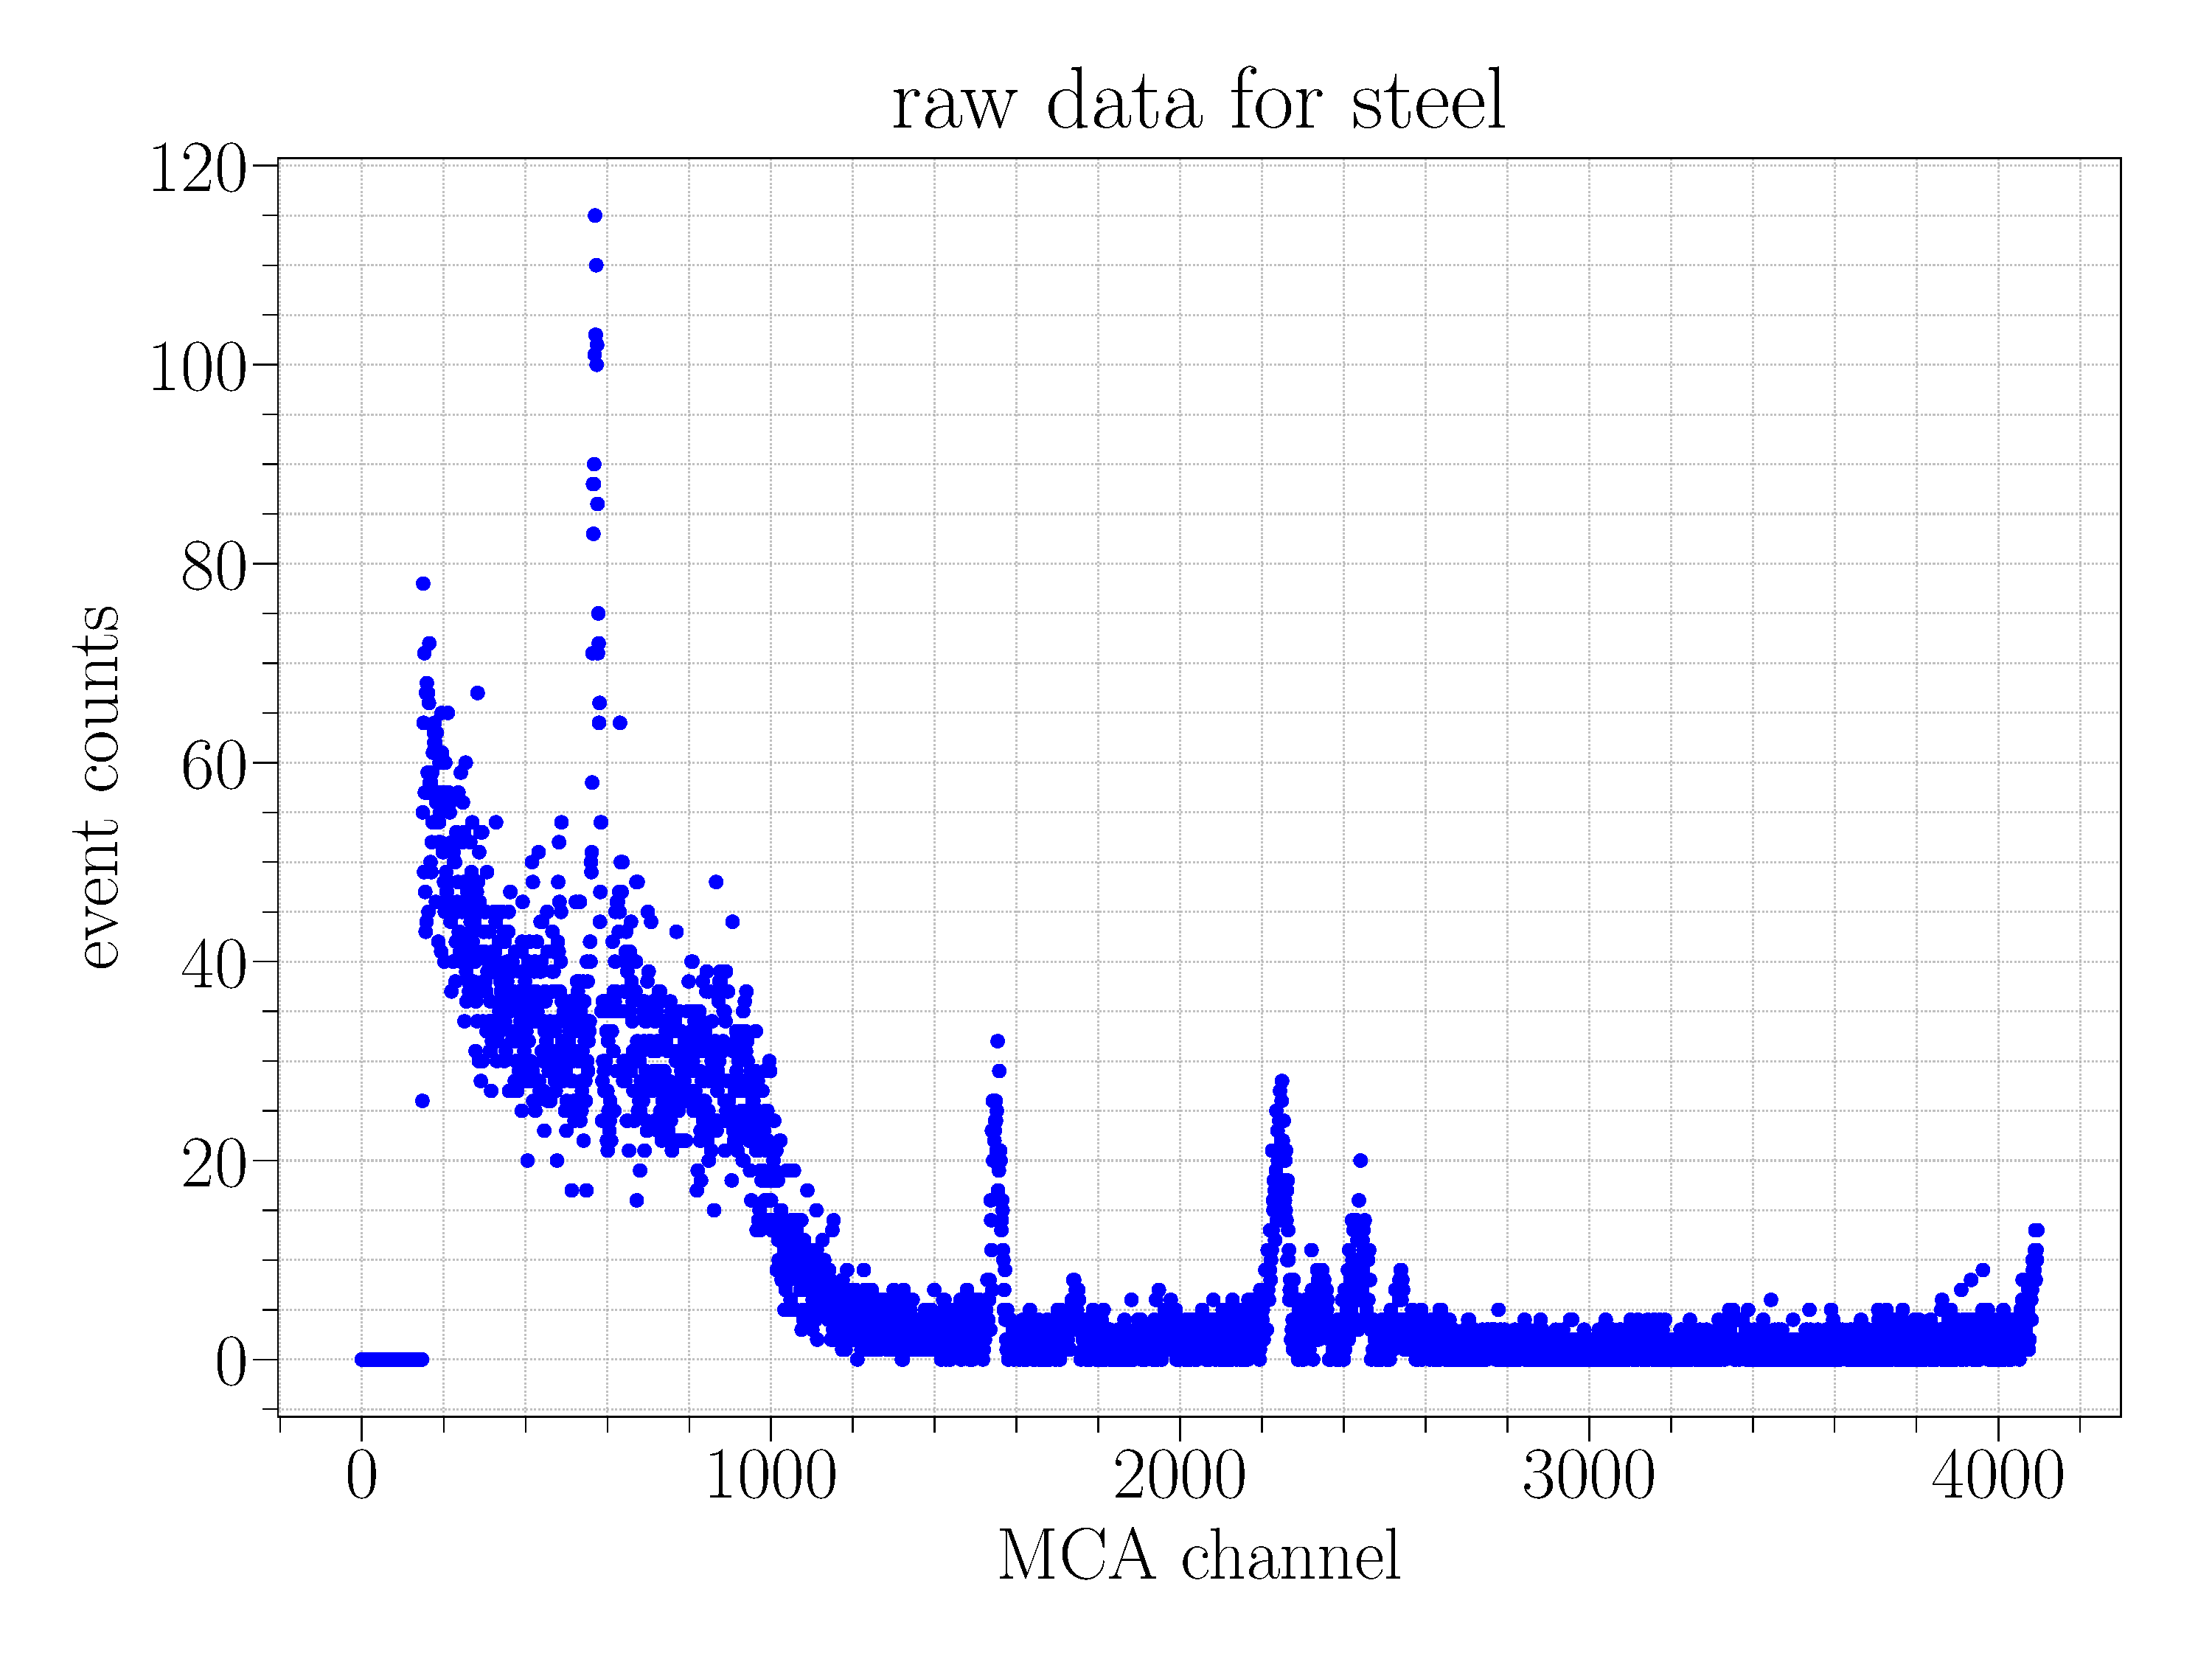
\includegraphics[scale=0.25]{../Figures/am_fe_raw.pdf}
\caption{Rohdaten für die Edelstahlprobe}
\label{am_fe_raw}
\end{figure}

\begin{figure}[H]
\centering
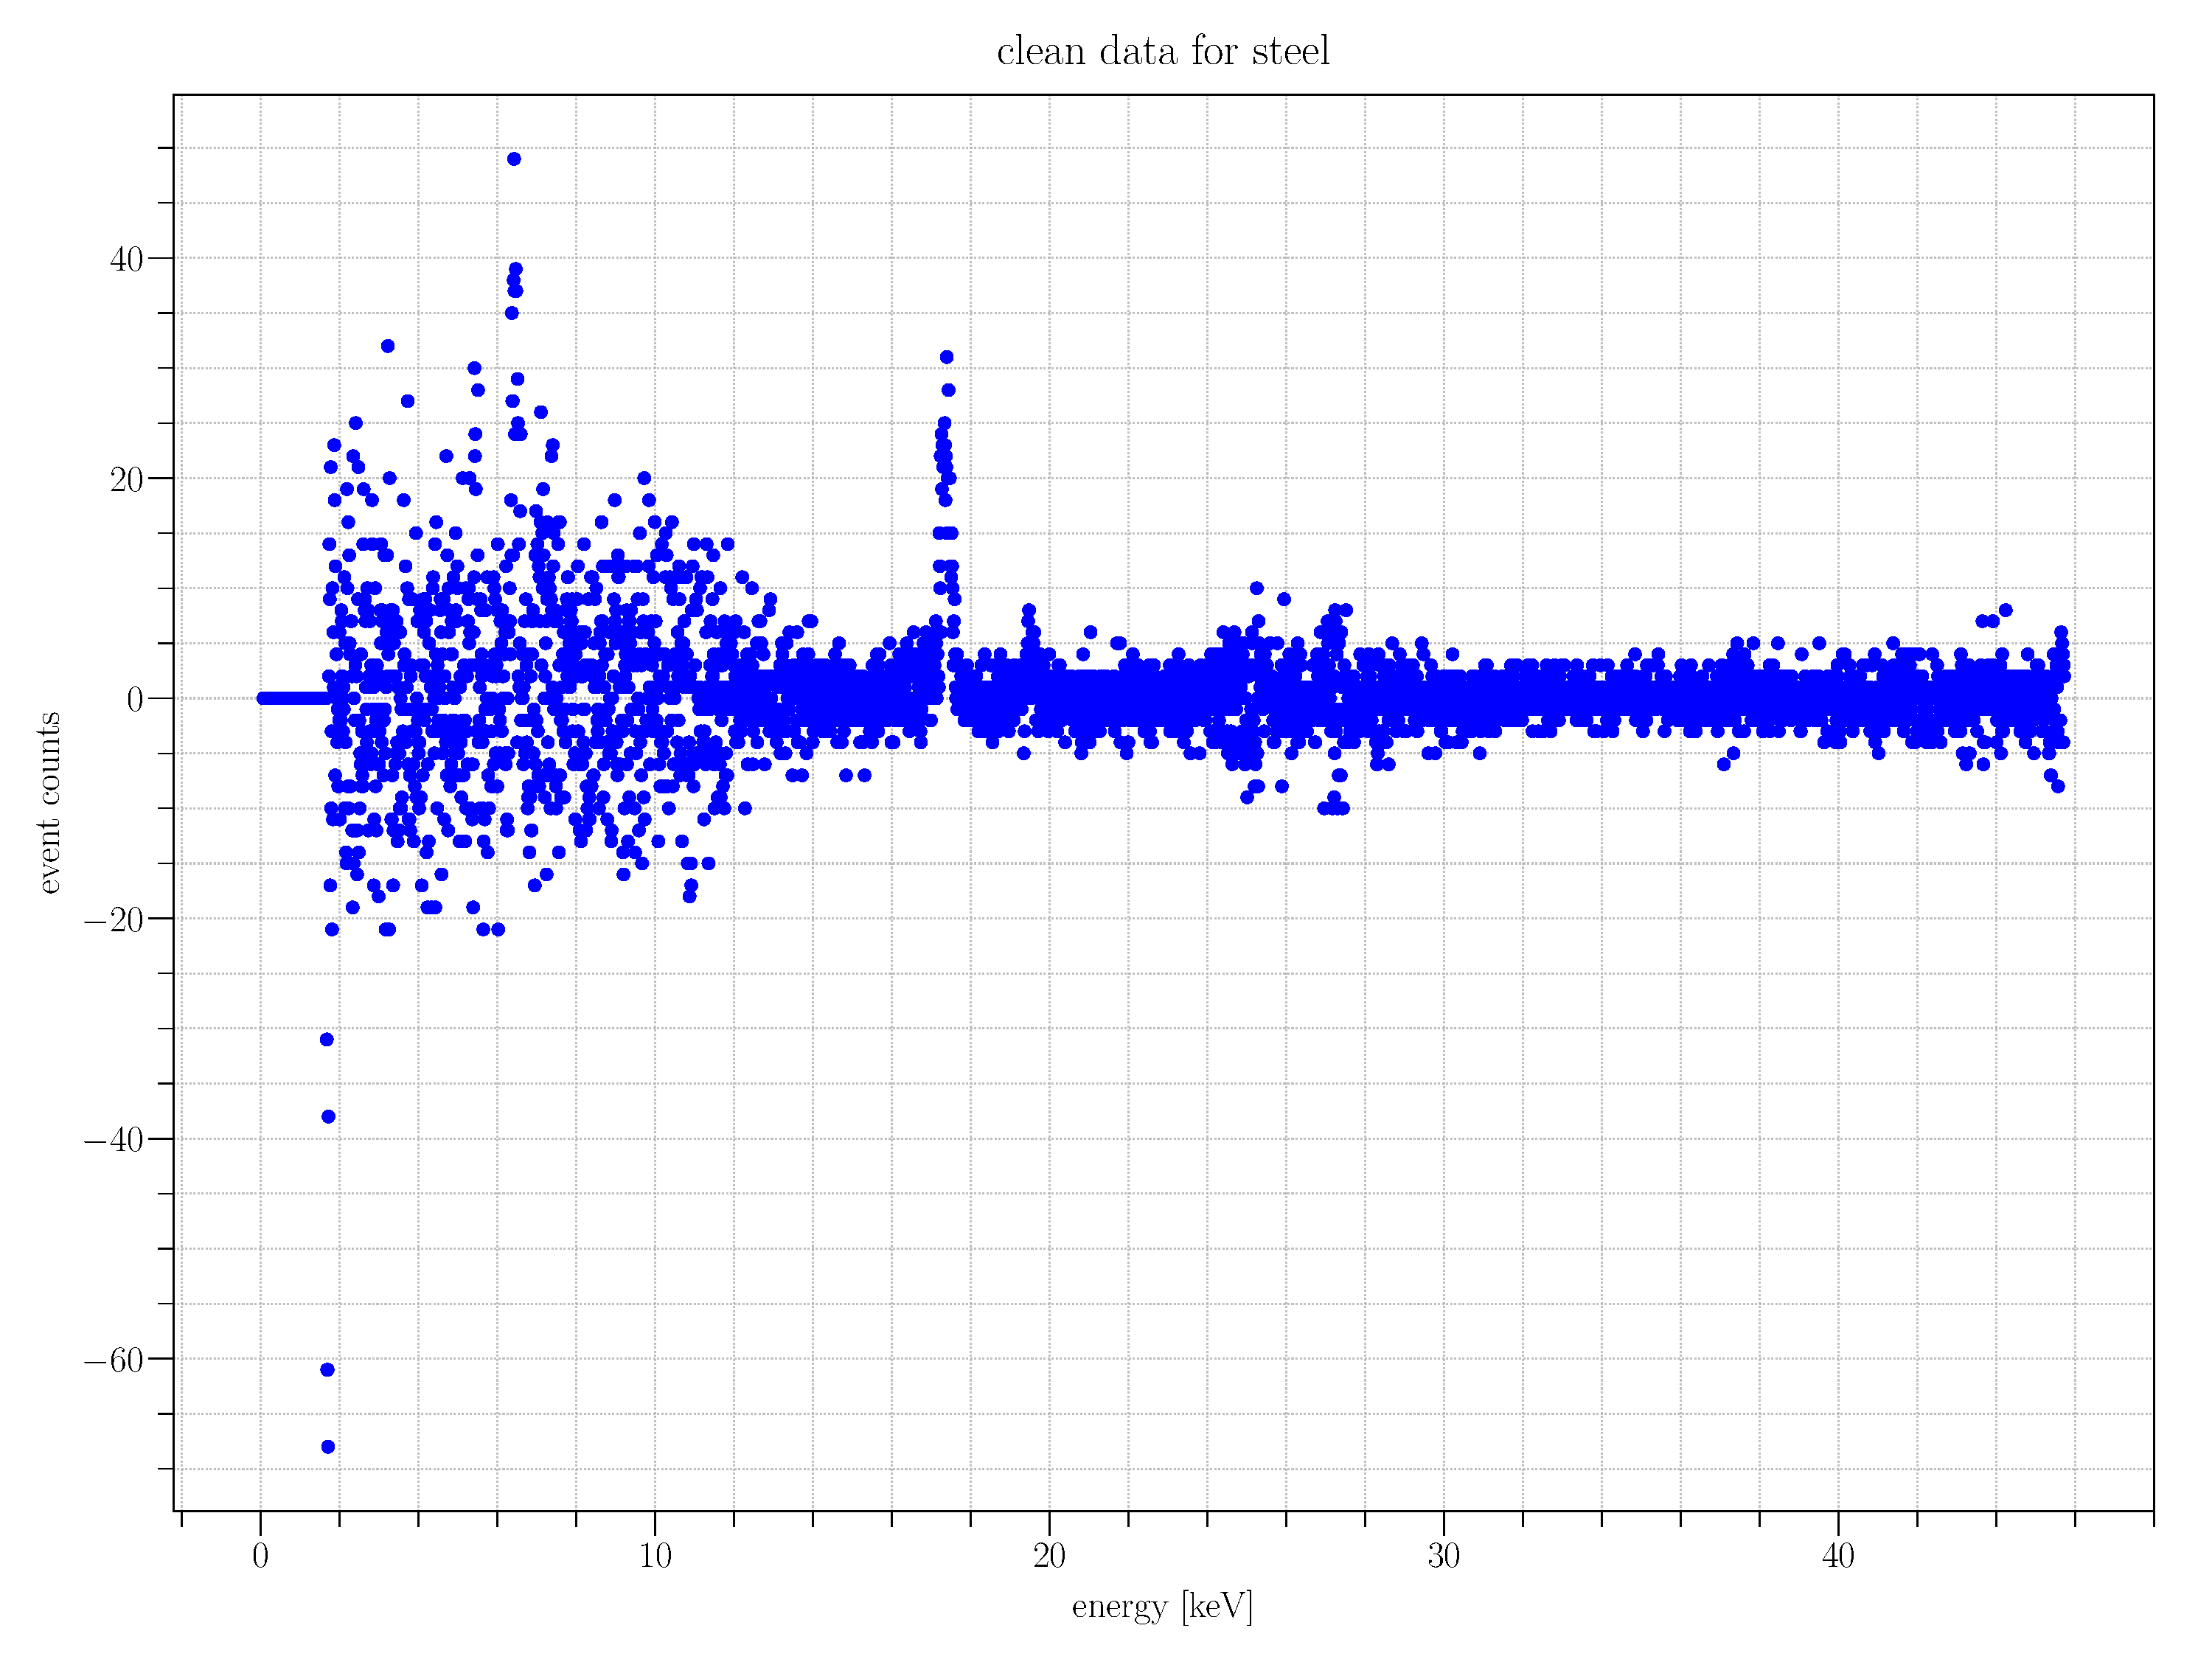
\includegraphics[scale=0.25]{../Figures/am_fe_clean.pdf}
\caption{Daten für die Edelstahlprobe nach Abzug der Leermessung und Kalibration}
\label{resolution}
\end{figure}

Trotz des starken Rauschens für geringe Energien, ist ein Peak sichtbar der heraussticht bei etwa 6 keV, von dem wir vermuten es könnte sich um die $K_\alpha$-Linie handeln. Außerdem fällt deutlich ein weiterer Peak bei etwa 17 keV auf. Wir ermitteln jeweils den Mittelwert und dessen Fehler beider Peaks, wieder durch Anpassung einer Gaußkurve.

\begin{table}[H]
	\renewcommand{\arraystretch}{1.5}
	\centering
	\begin{tabular}{|c|c|c|c|}
		\hline
		Vermutete Linie & erwarteter Wert & gemessener Wert & Abweichung \\
		\hline
		$K_\alpha$ & \SI{6.403}{keV} & $(6.442 \pm 0.003 \pm 0.037)$keV & $1,051\sigma$ \\
		\cline{1-4}
		 & & $(17.368 \pm 0.006 \pm 0.053)$keV & \\
		\hline
	\end{tabular}
	\caption{Ergebnisse der Analyse von Edelstahl.}
	\label{tab:am_fe_mean}
\end{table}

Die Ergebnisse legen Nahe, dass das Edelstahlplättchen tatsächlich hauptsächlich aus Eisen besteht.

\subsubsection{Energieauflösung}
Hier wollen wir die Energieauflösung des Detektors betrachten. Dafür schauen wir uns die Peaks an die wir bereits bei der Kalibration genutzt hatten. Diesmal brauchen wir deren Halbwertsbreiten $\Delta E$ die sich mit
\begin{equation}
	\Delta E = 2 \sqrt{2 \log2} \cdot \sigma
\end{equation}
aus den Standardabweichungen $\sigma$ ergeben. Letztere bekommen wir aus den entsprechenden Gaußfits.

Trägt man die Auflösung $\frac{\Delta E}{E}$ über die Energie auf, erkennt man wie erwartet einen stetigen Abfall (etwa $\frac{1}{E}$).

\begin{figure}[H]
\centering
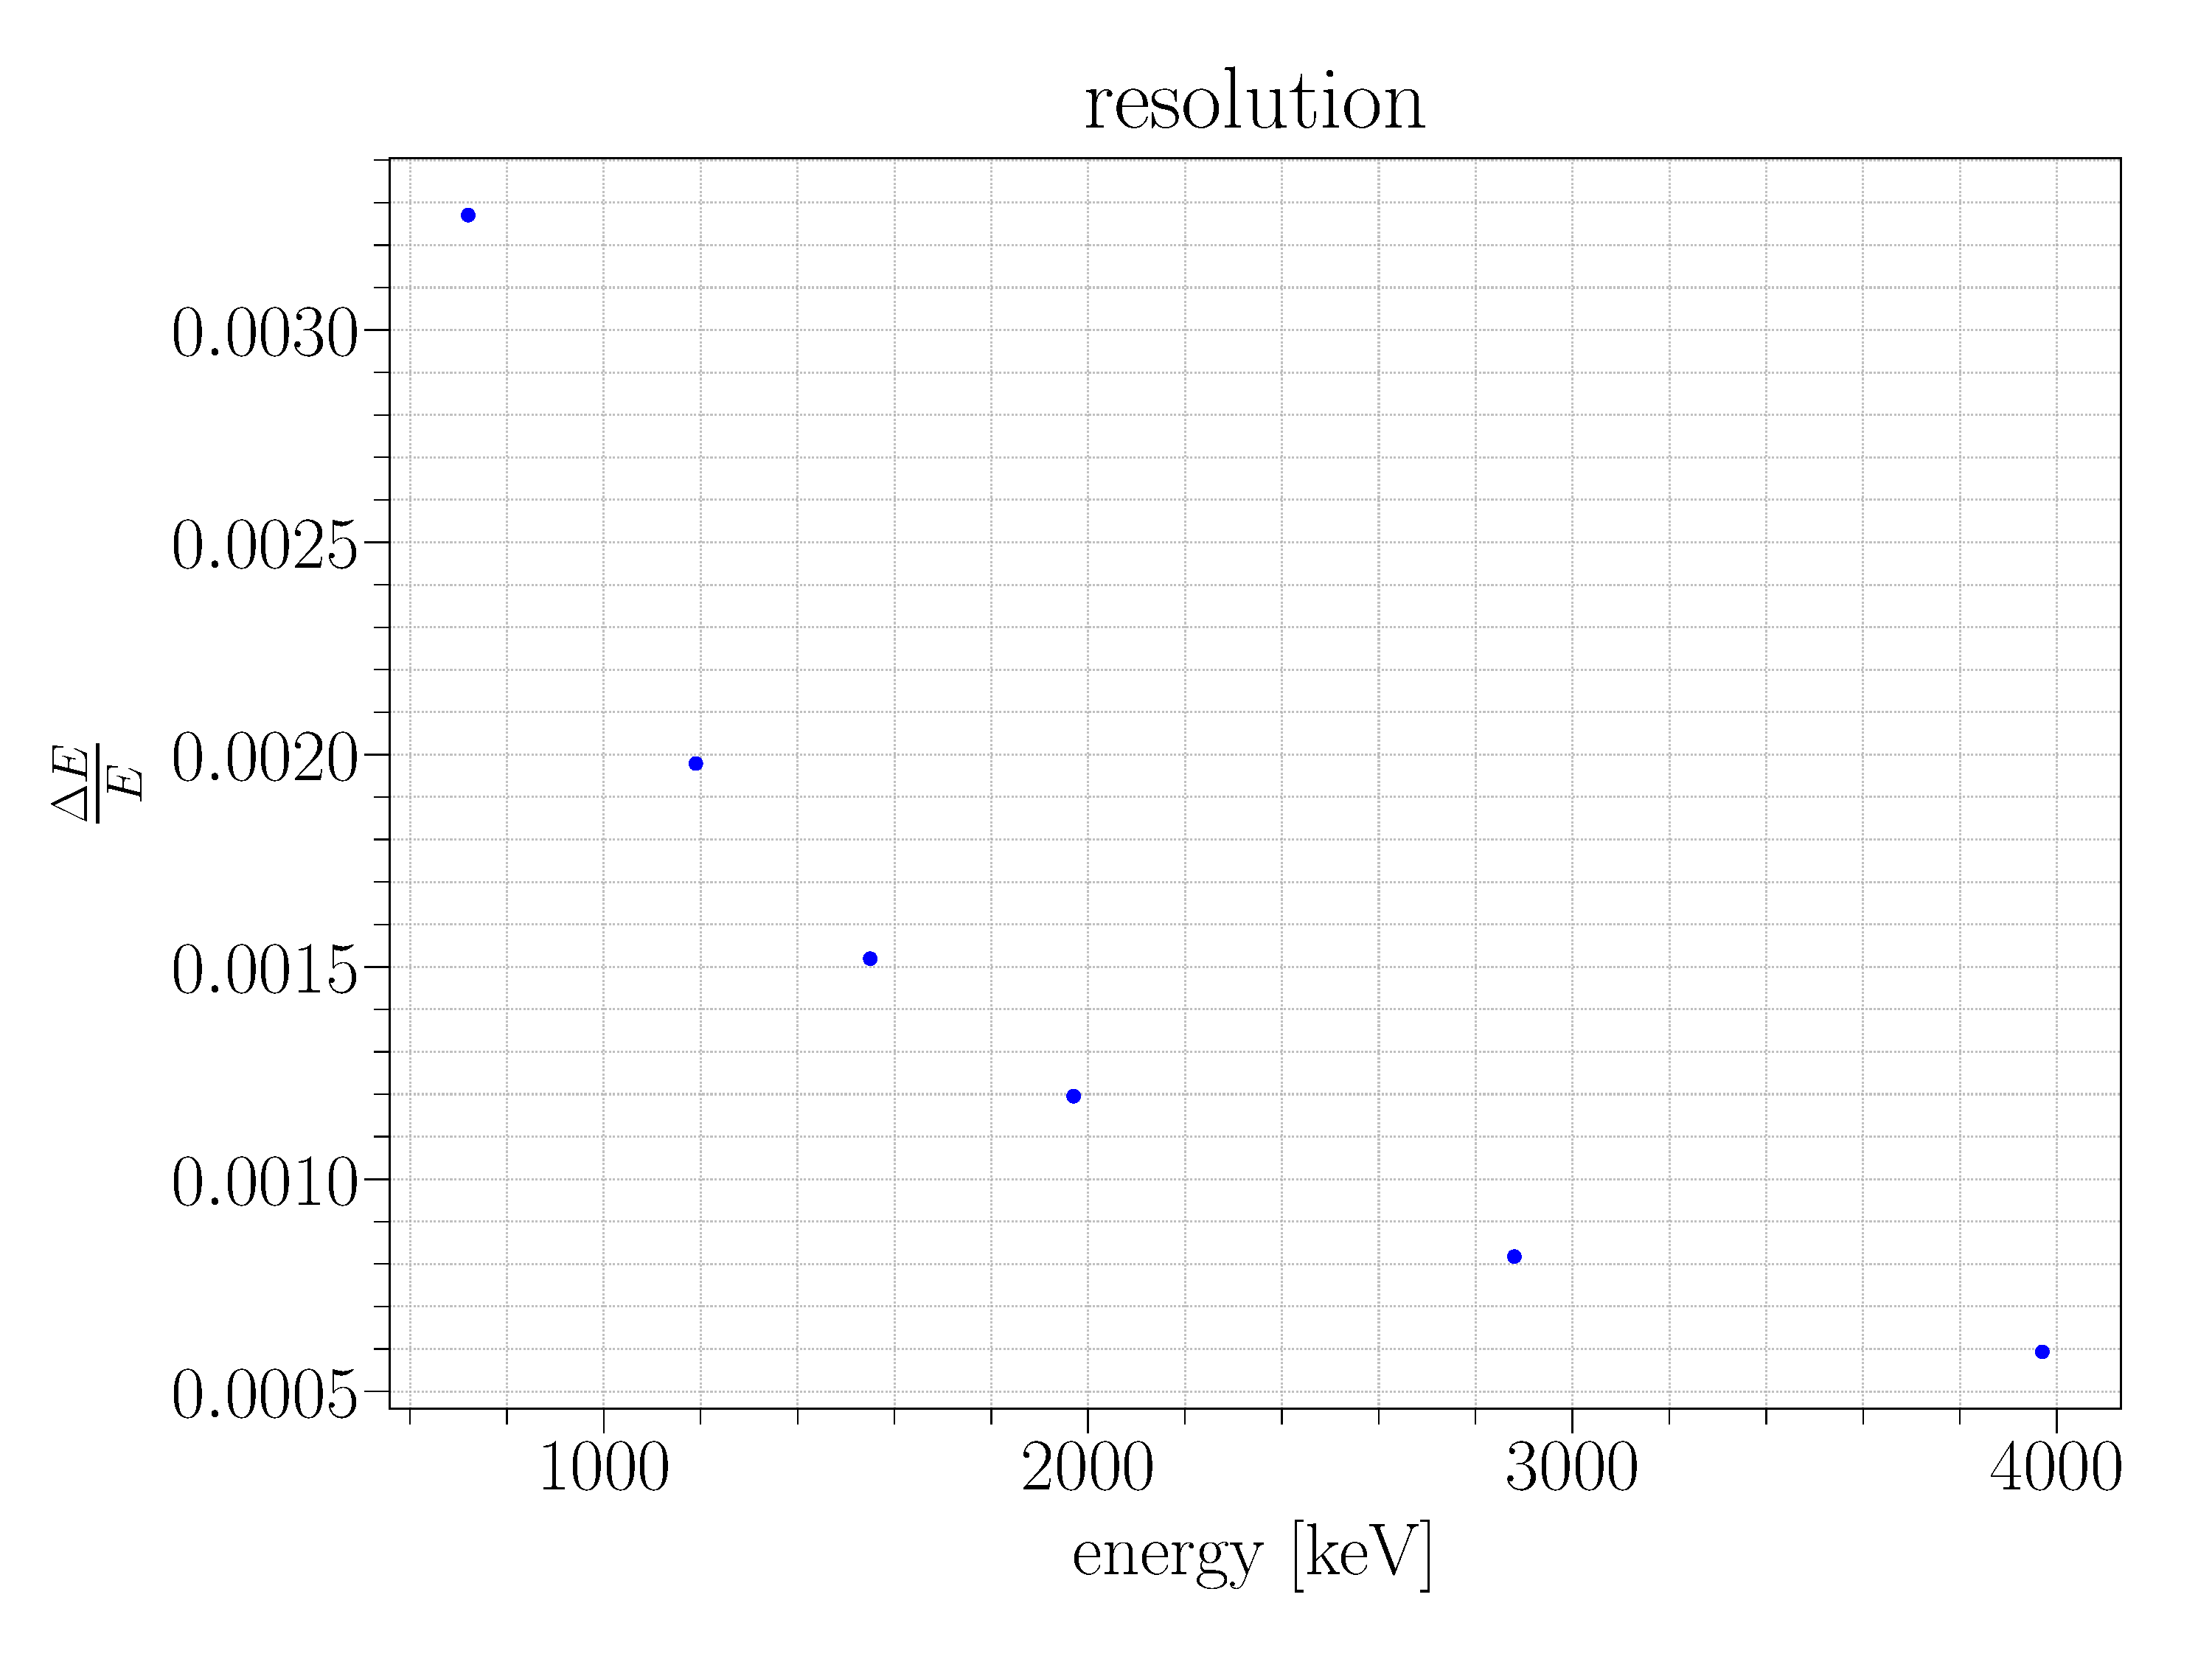
\includegraphics[scale=0.25]{../Figures/am_resolution.pdf}
\caption{Energieauflösung aufgetragen über die Energie}
\label{am_resolution}
\end{figure}

\section{Aufbau mit Röntgenröhre}
\subsection{Aufbau}
In diesem Aufbau nutzen wir eine Röntgenröhre. Die Probe wird in eine abgeschirmte Kammer gelegt, sodass sie von schräg unten von der Röngenröhre beschossen wird und die Röntgenstrahlung die in der Probe entsteht möglichst direkt in den ebenfalls darunter liegendem Detektor fällt. Die Kalibration wird hier durchgeführt mit Molybdän-, Kupfer- und Silberproben.

Anschließend analysieren wir ein Stein, ein Schneckengehäuse, ein Computerchip, eine Tablette, ein Bleiblock, eine 10-cent-Münze, und eine Batterie.

\subsection{Auswertung}
\
\section{Fazit}

\section{Anhang}
	
	
\end{document}